\section{Analysis}

This section introduces the used dataset in detail. \ref{sec2.1} subsection introduces the structure of the provided dataset. In \ref{sec2.2} we provide a thorough insight into the data mainly through visualization. Here the features and anomalies which will have to be cured are shown. In \ref{sec2.3} we provide the set of algorithms which will be used for this purpose and finally in \ref{sec2.4} we provide a benchmark model, with which our solution is going to be compared.

\subsection{Data Structure}\label{sec2.1}

The provided dataset is stored in 3 '.json' files: 'profile.json', 'portfolio.json' and 'transcript.json'. 
\subsection*{profile.json}
The profile.json file contains personal data about costumers in the following fields (17000 costumers):
\begin{itemize}
	\item gender: (categorical) M, F, O or null
	\item age: (numeric) missing value encoded as 118
	\item id: (string/hash)
	\item became\_member\_on: (date) format YYYYMMDD
	\item income: (numeric)
\end{itemize}

\begin{figure}[h]
	\centering
	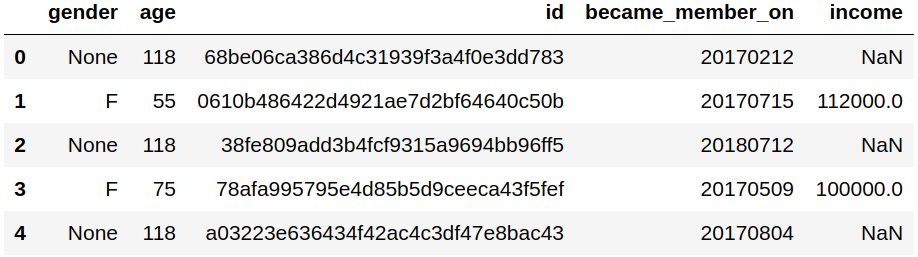
\includegraphics[width=0.8\textwidth]{fig/profile_head.jpg}
	\vspace*{-0.1in}
	\caption{Sample from the portfolio dataset}
	\label{fig1}
	\vspace*{-0.2in}
	\bigskip
\end{figure}

\subsection*{portfolio.json}
The portfolio.json file contains the data of the offers sent during the test period in fields (10 offers): 
\begin{itemize}
	\item reward: (numeric) money awarded for the amount spent
	\item channels: (list) web, email, mobile, social
	\item difficulty: (numeric) money required to be spent to receive reward
	\item duration: (numeric) time for offer to be open, in days
	\item offer\_type: (string) BOGO, discount, informational
	\item id: (string/hash)
\end{itemize}

\begin{figure}[h]
	\centering
	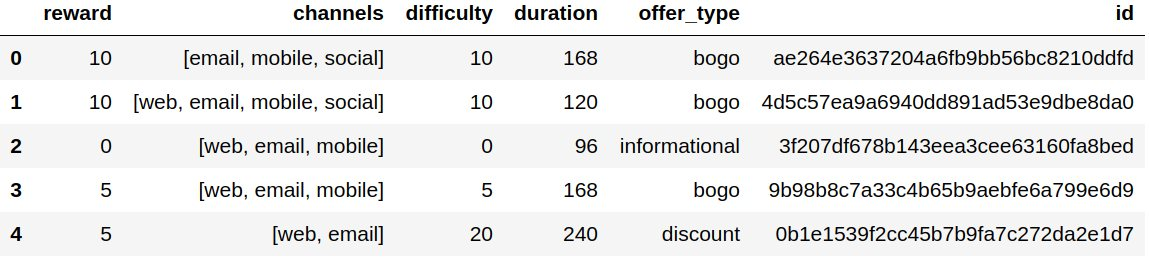
\includegraphics[width=0.7\textwidth]{fig/portfolio_head.jpg}
	\vspace*{-0.1in}
	\caption{Sample from the profile dataset}
	\label{fig2}
	\vspace*{-0.2in}
	\bigskip
\end{figure}

\subsection*{Transcript.json}
The transcript.json file contains timestamped data about transaction and offers in the following fields ((306648 events):
\begin{itemize}
	\item person: (string/hash)
	\item event: (string) offer received, offer viewed, transaction, offer completed
	\item value: (dictionary) different values depending on event type
	\subitem offer id: (string/hash) not associated with any "transaction"
	\subitem amount: (numeric) money spent in "transaction"
	\subitem reward: (numeric) money gained from "offer completed"
	\item time: (numeric) hours after start of test
\end{itemize}

\begin{figure}[h]
	\centering
	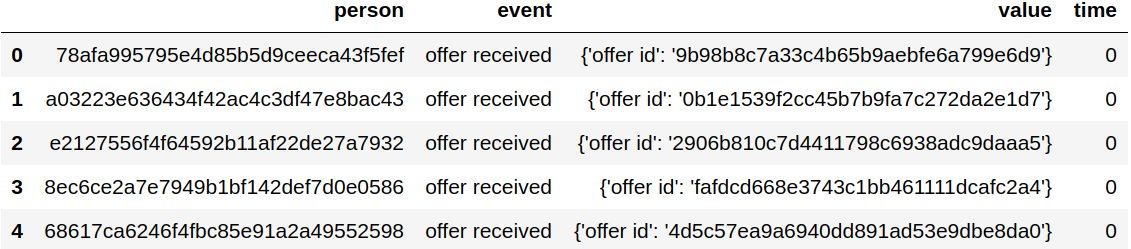
\includegraphics[width=0.9\textwidth]{fig/transcript_head.jpg}
	\vspace*{-0.1in}
	\caption{Sample from the transcript dataset}
	\label{fig3}
	\vspace*{-0.2in}
	\bigskip
\end{figure}

This data in itself is not very informative, so serious effort has to be made to extract meaningful features from it. The feature extraction / engineering is going to be shown in section \ref{sec3}

\subsection{Data Exploration}\label{sec2.2} 

\subsubsection{Dealing with missing values}
As it can be seen in Figure \ref{fig1}, the portfolio dataset is not complete. By examining the data we have established that there are two kinds of data points: One in which all data is provided and one in which gender, age and also income is missing. This can be due to several reasons, one of which is that these people did not agree with the company's privacy policy.

A total number of 2175 datapoints are effected by missing values. One have to deal with these datapoints. A potential solution would be to discard these datapoints from the dataset. However these people possibly form an interesting group in the dataset, so we decided to keep these datapoints as well. These datapoints will be clearly differentiated from the other datapoints by giving them a gender 'U' (unknown). The age and income values will be filled with the respective mean values. The unknown gender category seems to be a reasonable choice for the following reason: Filling up the missing values with the respective means seriously changes data distribution. By the extra gender group we hope to separate these points from all the other ones sufficiently.

\subsubsection{Profile Data Exploration}
There are 8484 Male and 6129 Female datapoints in the dataset. In this respect the number male and female datapoints is quite well balanced, so no care has to be taken on compensating it in any direction. The number of people who classify themselves into other genders is however very small. These people are decided to be kept in the dataset but we assume that the predictions on them will not be very accurate.

The membership length is calculated for the people counting from the date of the last person who got a membership. This is an arbitrary choice, however since we are only interested in the relative lengths of the memberships (the data is going to be normalized / standardized) it works totally fine. After this, the age, income and membership length distribution of the costumers can be analyzed. These distributions, also separated based on genders can be seen in Figure \ref{fig4}.

\begin{figure}[h]
	\centering
	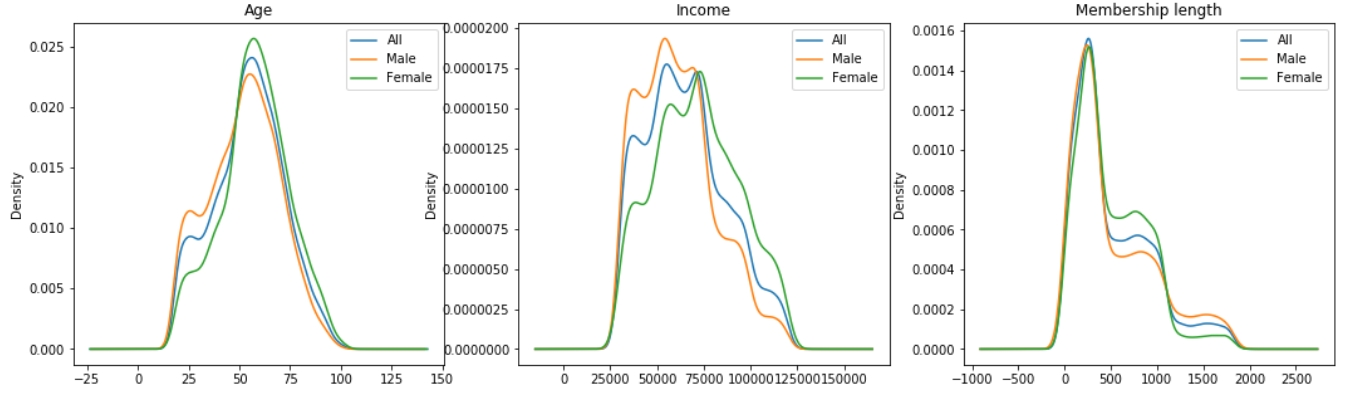
\includegraphics[width=0.99\textwidth]{fig/profile_distributions.jpg}
	\vspace*{-0.1in}
	\caption{Distributions of the age, income and membership data in the dataset}
	\label{fig4}
	\vspace*{-0.2in}
	\bigskip
\end{figure}

From the above plots we derive the following conclusions:
\begin{itemize}
	\item The age distribution is relative nice. It has got a small peak around 25 years, but we assume that it will not pose a serious problem during training.
	\item The income is not perfectly well distributed, it has got some local peaks at certain points. However it will possibly be sufficient for training. There are some differences between the male and female distributions. The male costumers tend to have lower income than the female costumers.
	\item The membership length on the other hand is quite badly distributed. It has a huge peak between 0 and 500. Other than that, there tend to be some intervals where the distribution is almost constant. This left skewed distribution will probably require some transformation before using it for training.
\end{itemize}

Based on these experiments we conclude that it will probably be sufficient to only standardize the age and income distributions and only the membership length data needs to be transformed to behave better during training.

\subsubsection{Offer Data Exploration}

For being able to explore the transcript data, first the field "value" has to be extracted. 3 new columns, called "offer\_id", "amount" and "reward" are created and are filled with the values from the "value" column's dictionaries. 

As it will be seen later, we mostly create our features from statistical data about the offers the costumers receive. For this reason firs we observed some properties of the offers related data in the transcript dataset. We checked the number of received, viewed and completed offers from each type. (From now on we use the phrase "offer" both for actual offers and for simply informational material.) Obviously an informational material can not be completed, however it can be viewed. The distributions can be seen in Figure \ref{fig5}. (The numbers 0-9 correspond to different offers. These were assigned to the offers based on their order in the portfolio dataset)

\begin{figure}[h]
	\centering
	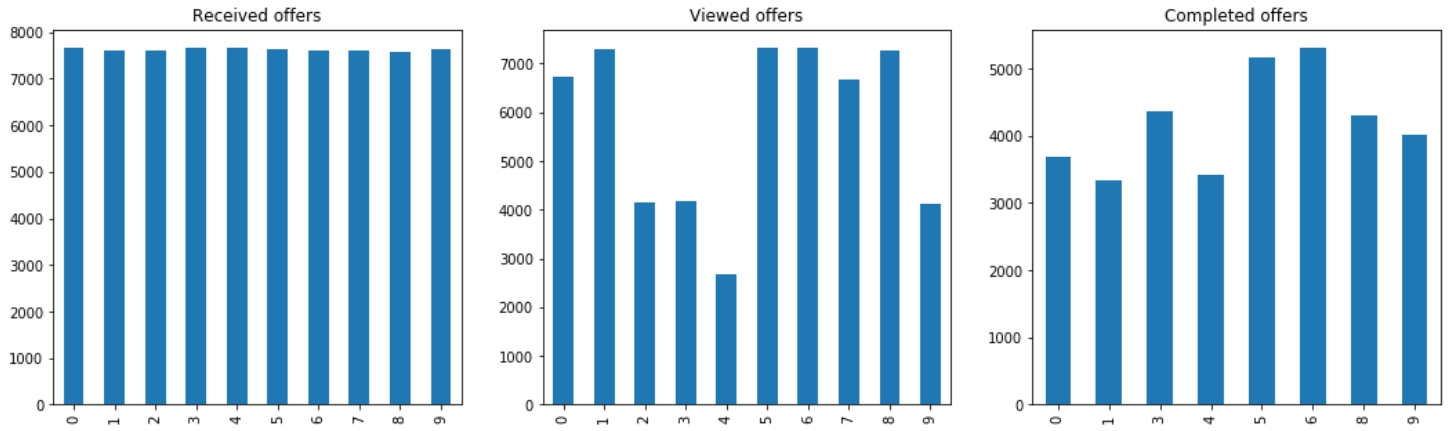
\includegraphics[width=0.99\textwidth]{fig/offer_distributions_1.jpg}
	\vspace*{-0.1in}
	\caption{Number of offers received, viewed and completed}
	\label{fig5}
	\vspace*{-0.2in}
	\bigskip
\end{figure}

The following observations can be made based on these figures:
\begin{itemize}
	\item The amount of sent out promotions is almost the same for every offer type.
	\item The amount of viewed promotions varies stronger and by far the least people viewed the promotion with the highest difficulty and longest duration.
	\item The completion is also relatively homogeneous. (The offer types 2 and 7 correspond to the informational type offers which can not be completed, hence these are missing from the table.)
\end{itemize}

After this we have examined how the distribution of the success of the offers look like. For this we have calculated for every person in the dataset, how many times he/she a) viewed, b) viewed and completed and c) not viewed but still completed an offer. The resultant numbers can be examined in Figure \ref{fig6}. (The x axis of the plots represent the amount of offers per person that fulfills the property indicated in the plot title and the y axis represents the number of people.)

\begin{figure}[h]
	\centering
	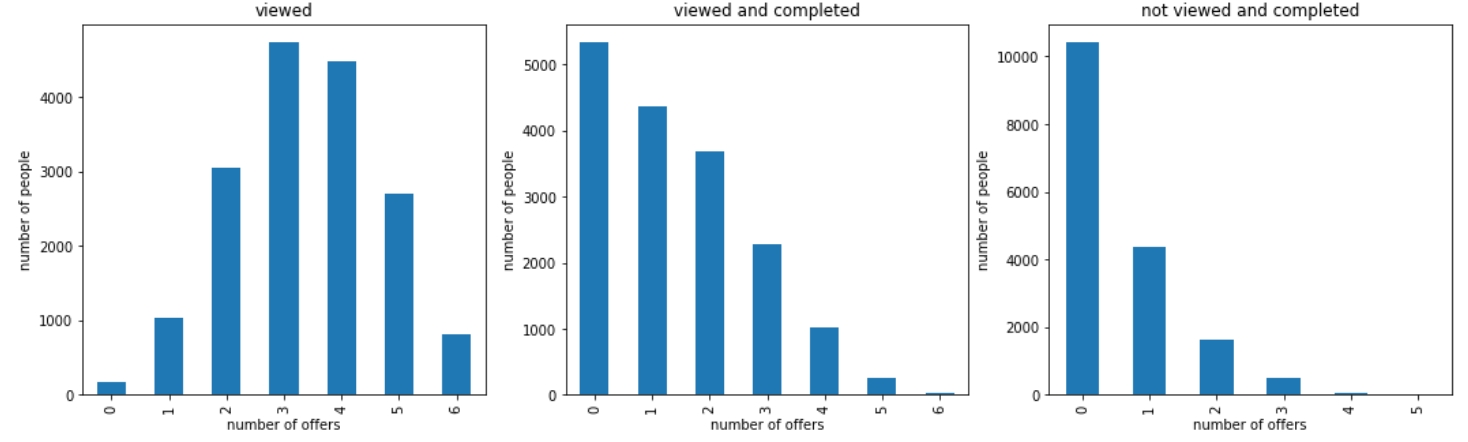
\includegraphics[width=0.99\textwidth]{fig/offer_distributions_2.jpg}
	\vspace*{-0.1in}
	\caption{Sample from the transcript dataset}
	\label{fig6}
	\vspace*{-0.2in}
	\bigskip
\end{figure}

These plots look quite like what we expected:
\begin{itemize}
	\item The number of viewed offers is quite normally distributed. It is not very common that people never look at offers not that they view every single offer they receive.
	\item The number of people who view and then complete an offer several times decreases linearly with the number of occurrences.
	\item  The number of people who view and then complete an offer several times decreases in an exponential-like fashion. It is very improbable, that someone would complete several offers accidentally without knowing about the offer. 
\end{itemize}

\subsubsection{Transaction data Exploration}
A huge part of the transcript dataset are transactions. In the followings we derive some conclusions about these data.

During exploration of the transactions data we have quickly realized that there are some outliers which seriously distort the statistics about the data. The issue can easily be seen in Figure \ref{fig7} where the distribution of the amount of a single transaction is shown:
\begin{figure}[h]
	\centering
	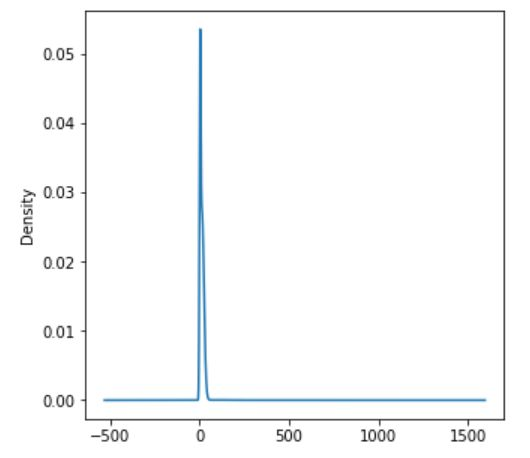
\includegraphics[width=0.4\textwidth]{fig/transaction_distribution_1.jpg}
	\vspace*{-0.1in}
	\caption{Effect of outlier transaction}
	\label{fig7}
	\vspace*{-0.2in}
	\bigskip
\end{figure}

There is an outlier transaction with an amount of 1062.28\$ although the mean for the whole dataset is around 12.7\$. Most of the data is in a normal range, however there are some unlikely high values in the dataset.

A very similar can be said about the cumulative amount of money a person sent during the 30 day period. The mean value for the cumulative spent amount is around 104\$, however the maximum value is 1608\$. Also there are a total number of 422 people who did not spend any money during this period. In Table \ref{table1} we show the number of people who spent more than a specified threshold.

\begin{table}[h] \label{table1}
	\begin{center}
	\begin{tabular}{ c | c | c | c | c | c | }
		& $>100$ & $>200$ & $>300$ & $>500$ & $>1000$\\
		\hline
		number of people & 6722 & 2349 & 738 & 272 & 48 \\
		\hline  
	\end{tabular}
	\end{center}
	\caption{Number of people in the dataset who spent more than different thresholds during the 30 days.}
\end{table}

We decided that some people should be excluded from the data for the following two reasons:
Either they are not representative for the whole group, or they are not the target who the company should consider when they plan their advertisement campaign. By not being representative we mean, that a portion of the group spends much more money than the rest of the group. They are outliers in the dataset and would just reduce the performance of the model. The second group is the people who have not spent any money during the 30 day period. These people should not be considered as potential costumers and hence can be discarded from the dataset. 

In Figure \ref{fig8} the distribution of the cumulative amount spent by a person can be seen if a group of people whose purchases are over a specified threshold are discarded from the data.

\begin{figure}[h]
	\centering
	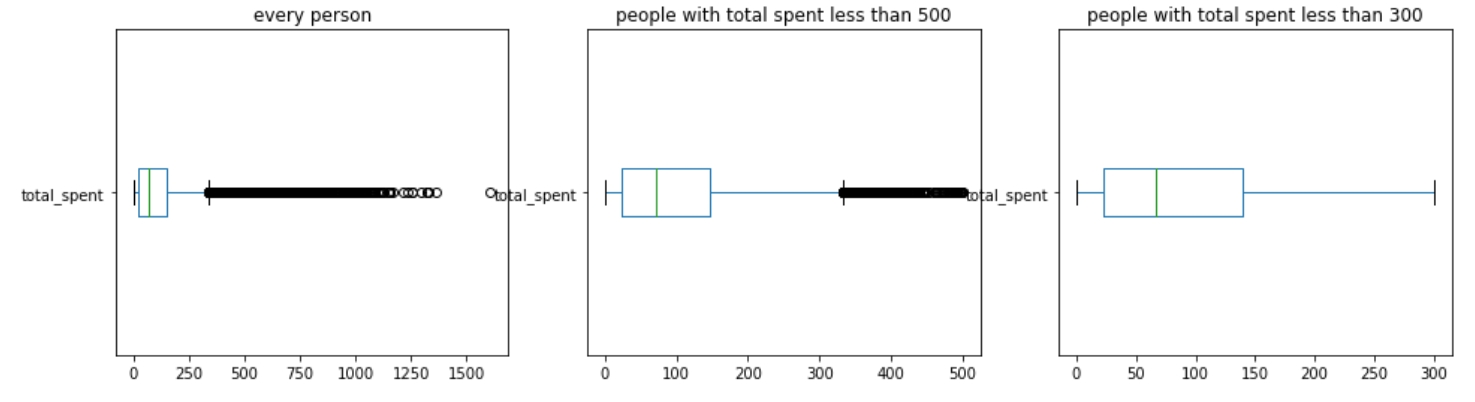
\includegraphics[width=0.99\textwidth]{fig/transaction_distribution_2.jpg}
	\vspace*{-0.1in}
	\caption{Distribution of cumulative money spent during the 30 day period}
	\label{fig8}
	\vspace*{-0.2in}
	\bigskip
\end{figure}

On the first two figures one can see the effect of outlier data in the dataset. Based on these experiments we have decided to discard the people (and all data related to them) from the dataset, who either have spent 0\$ or more than 300\$ during the 30 day period. This means that a total number of 1160 people will be dropped from the data. This is only 6.8\% of the people and we assume that around the same amount of data will be lost from the transcript dataset.

\subsection{Algorithms and Techniques}\label{sec2.3}

It is a crucial step to preprocess the data that later will be fed to the model during training. To be able to decide which preprocessing steps are required for which features data visualization is unavoidable. After we have obtained some characteristics of the data through visualization we concluded that the following algorithms are going to be use through preprocessing:

The age and income features are relatively nicely distributed and hence will only have to be standardized. We would like to carry out the standardization before filling up the missing values with the respective means, since otherwise these would distort the data strongly. We have chosen sklearn's StandarScaler algorithm since it is able not to consider "None" type values. The scaler standardizes the data using the following formula:
$$x_{scaled} = \frac{x - \mu}{\sigma}$$
where $\mu$ is the mean and $\sigma$ is the standard deviation of the feature calculated for the whole dataset.

The membership length is a strongly left skewed distribution and hence has to be transformed. For this we have chosen to use sklearn's QuantileTransform algorithm. This method transforms the features to follow a uniform or a normal distribution using quantiles information. Therefore, for a given feature, this transformation tends to spread out the most frequent values.

Due to the reasons detailed in the previous subsections, the people and all data related to them, who tend to be outliers because of their spending are going to be removed from the dataset.

An important part of the solution that we have chosen is the generation of training data from the provided dataset. This algorithm is going to be detailed later in the Methodology section.

\subsubsection{Chosen model}

we are going to train a feed forward neural network to predict into which category an offer is going to fall after it is sent to a costumer. Feed forward neural networks are relatively easy to train and are universal approximators in the sense, that an infinitely complex neural network can approximate any given nonlinear function. This does not necessarily mean that neural networks are the best choice for every task. However they are quite usual choices for data where one suspects very tricky underlying distribution as it is in this case. 

The neural network is going to be implemented using the PyTorch framework.

\subsection{Banchmark Model}\label{sec2.4}

We have chosen an easily implementable and easy to evaluate model as benchmark model. A kNN (k Nearest Neighbor) model is going to be used. As we suspect that similar people react similarly to offers a kNN classifier will possibly perform quite well for the task and hence will be a good benchmark model to compare the performance of the neural network to.



